% WR figure exported by sim_ui.py -- 2026-09-18 21:53:26
%
% Preamble (once, in your thesis):
%   \usepackage{pgfplots}
%   \pgfplotsset{compat=1.18}
%
% Use:
%   \begin{figure}[htbp]\centering
%     \input{wr_convergence}
%     \caption{...}\label{fig:...}
%   \end{figure}
%
% \input nests (unlike \include), so this works inside a chapter file the root
% already \includes. Pasting the body below inline works too -- the \definecolor
% lines may then be hoisted into the preamble and dropped from each figure.
%
% Series are thinned to ~2000 points each (min/max decimation, so spikes are
% preserved); edit _PGF_MAX_PTS in sim_ui.py for the full-resolution data.
%
% Run: coupling_mode=voltage-driven; precondition=on (optimized); interface_form=Thevenin (V source); use_t_floor=bare dt; interface_consistency=BDF-1/BE (naive); N_field_windows=80; N_xyce_samples=200; xyce_integration_method=Backward-Euler (maxord=1)

\definecolor{C0}{HTML}{1F77B4}
\definecolor{C1}{HTML}{FF7F0E}
\definecolor{C2}{HTML}{2CA02C}
\definecolor{C3}{HTML}{D62728}

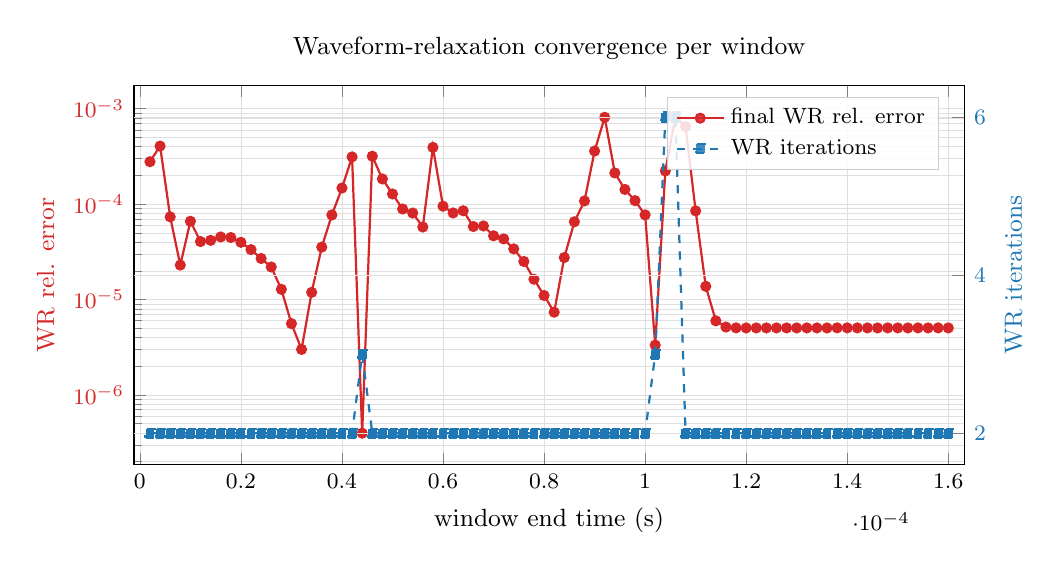
\begin{tikzpicture}
\begin{axis}[
  width=\linewidth,
  height=6.4cm,
  title={Waveform-relaxation convergence per window},
  xlabel={window end time (s)},
  ylabel={WR rel. error},
  grid=both,
  grid style={line width=.2pt, draw=gray!25},
  legend pos=north east,
  legend cell align=left,
  legend style={font=\footnotesize, fill=white, fill opacity=0.85, text opacity=1, draw=gray!40},
  tick label style={font=\footnotesize},
  label style={font=\small},
  title style={font=\small},
  scaled x ticks=true,
  xmin=-1.16e-06,
  xmax=0.00016316,
  ymode=log,
  axis y line*=left,
  ylabel style={color=C3},
  yticklabel style={color=C3}
]
  \addplot[color=C3, line width=0.8pt, mark=*, mark size=1.6pt] coordinates {
    (2e-06,0.0002781) (4e-06,0.0004054) (6e-06,7.353e-05) (8e-06,2.296e-05) (1e-05,6.609e-05) (1.2e-05,4.051e-05)
    (1.4e-05,4.169e-05) (1.6e-05,4.528e-05) (1.8e-05,4.465e-05) (2e-05,3.978e-05) (2.2e-05,3.335e-05) (2.4e-05,2.691e-05)
    (2.6e-05,2.194e-05) (2.8e-05,1.28e-05) (3e-05,5.594e-06) (3.2e-05,3.001e-06) (3.4e-05,1.189e-05) (3.6e-05,3.543e-05)
    (3.8e-05,7.694e-05) (4e-05,0.0001473) (4.2e-05,0.0003123) (4.4e-05,3.978e-07) (4.6e-05,0.0003173) (4.8e-05,0.0001834)
    (5e-05,0.0001277) (5.2e-05,8.88e-05) (5.4e-05,8.058e-05) (5.6e-05,5.751e-05) (5.8e-05,0.0003929) (6e-05,9.499e-05)
    (6.2e-05,8.078e-05) (6.4e-05,8.51e-05) (6.6e-05,5.82e-05) (6.8e-05,5.901e-05) (7e-05,4.653e-05) (7.2e-05,4.318e-05)
    (7.4e-05,3.392e-05) (7.6e-05,2.504e-05) (7.8e-05,1.633e-05) (8e-05,1.102e-05) (8.2e-05,7.372e-06) (8.4e-05,2.754e-05)
    (8.6e-05,6.523e-05) (8.8e-05,0.0001079) (9e-05,0.0003596) (9.2e-05,0.0008117) (9.4e-05,0.000212) (9.6e-05,0.0001424)
    (9.8e-05,0.0001087) (0.0001,7.705e-05) (0.000102,3.329e-06) (0.000104,0.0002224) (0.000106,0.0008168) (0.000108,0.0006482)
    (0.00011,8.486e-05) (0.000112,1.375e-05) (0.000114,5.98e-06) (0.000116,5.148e-06) (0.000118,5.048e-06) (0.00012,5.04e-06)
    (0.000122,5.04e-06) (0.000124,5.041e-06) (0.000126,5.041e-06) (0.000128,5.041e-06) (0.00013,5.041e-06) (0.000132,5.041e-06)
    (0.000134,5.04e-06) (0.000136,5.038e-06) (0.000138,5.048e-06) (0.00014,5.046e-06) (0.000142,5.043e-06) (0.000144,5.041e-06)
    (0.000146,5.038e-06) (0.000148,5.046e-06) (0.00015,5.042e-06) (0.000152,5.038e-06) (0.000154,5.045e-06) (0.000156,5.04e-06)
    (0.000158,5.047e-06) (0.00016,5.041e-06)
  };
\end{axis}
\begin{axis}[
  width=\linewidth,
  height=6.4cm,
  title={},
  xlabel={},
  ylabel={WR iterations},
  grid=both,
  grid style={line width=.2pt, draw=gray!25},
  legend pos=north east,
  legend cell align=left,
  legend style={font=\footnotesize, fill=white, fill opacity=0.85, text opacity=1, draw=gray!40},
  tick label style={font=\footnotesize},
  label style={font=\small},
  title style={font=\small},
  scaled x ticks=true,
  xmin=-1.16e-06,
  xmax=0.00016316,
  axis y line*=right,
  axis x line=none,
  ylabel style={color=C0},
  yticklabel style={color=C0}
]
  \addlegendimage{color=C3, line width=0.8pt, mark=*, mark size=1.6pt}
  \addlegendentry{final WR rel. error}
  \addplot[color=C0, line width=0.8pt, dashed, mark=square*, mark size=1.6pt] coordinates {
    (2e-06,2) (4e-06,2) (6e-06,2) (8e-06,2) (1e-05,2) (1.2e-05,2)
    (1.4e-05,2) (1.6e-05,2) (1.8e-05,2) (2e-05,2) (2.2e-05,2) (2.4e-05,2)
    (2.6e-05,2) (2.8e-05,2) (3e-05,2) (3.2e-05,2) (3.4e-05,2) (3.6e-05,2)
    (3.8e-05,2) (4e-05,2) (4.2e-05,2) (4.4e-05,3) (4.6e-05,2) (4.8e-05,2)
    (5e-05,2) (5.2e-05,2) (5.4e-05,2) (5.6e-05,2) (5.8e-05,2) (6e-05,2)
    (6.2e-05,2) (6.4e-05,2) (6.6e-05,2) (6.8e-05,2) (7e-05,2) (7.2e-05,2)
    (7.4e-05,2) (7.6e-05,2) (7.8e-05,2) (8e-05,2) (8.2e-05,2) (8.4e-05,2)
    (8.6e-05,2) (8.8e-05,2) (9e-05,2) (9.2e-05,2) (9.4e-05,2) (9.6e-05,2)
    (9.8e-05,2) (0.0001,2) (0.000102,3) (0.000104,6) (0.000106,6) (0.000108,2)
    (0.00011,2) (0.000112,2) (0.000114,2) (0.000116,2) (0.000118,2) (0.00012,2)
    (0.000122,2) (0.000124,2) (0.000126,2) (0.000128,2) (0.00013,2) (0.000132,2)
    (0.000134,2) (0.000136,2) (0.000138,2) (0.00014,2) (0.000142,2) (0.000144,2)
    (0.000146,2) (0.000148,2) (0.00015,2) (0.000152,2) (0.000154,2) (0.000156,2)
    (0.000158,2) (0.00016,2)
  };
  \addlegendentry{WR iterations}
\end{axis}
\end{tikzpicture}
